\documentclass[
	letterpaper, % Paper size, specify a4paper (A4) or letterpaper (US letter)
	10pt, % Default font size, specify 10pt, 11pt or 12pt
]{CSUniSchoolLabReport}

%----------------------------------------------------------------------------------------
%	REPORT INFORMATION
%----------------------------------------------------------------------------------------

\title{Experiment One\\ Fundamentals of Electromagnetics Lab \\ EECE2530/1} % Report title

\author{Michael \textsc{Brodskiy}\\ \small \href{mailto:Brodskiy.M@Northeastern.edu}{Brodskiy.M@Northeastern.edu}}

\date{October 4, 2023} % Date of the report

%----------------------------------------------------------------------------------------


\begin{document}

\maketitle % Insert the title, author and date using the information specified above

\begin{center}
	\begin{tabular}{l r}
		Date Performed: & September 27, 2023 \\ % Date the experiment was performed
        Partners: & Manas \textsc{Mahajan} \& Priyam \textsc{Modi} \\ % Partner names
		Instructor: & Professor \textsc{Marengo-Fuentes} \\ % Instructor/supervisor
        TAs: & Nicolas \textsc{Casilli} \& Farah \textsc{Ben Ayed} \\ % Teachers Assistants 
	\end{tabular}
\end{center}

\newpage

\begin{abstract}

  The goal of this laboratory experiment is to familiarize oneself with the functions of a vector network analyzer, while, at the same time, applying knowledge of transmission lines and Smith chart analysis. This is done by plugging various components into the vector network analyzer and analyzing their Smith charts and phases.

\end{abstract}

\begin{flushleft}

  \textsc{Keywords:} \underline{vector network analyzer}, \underline{transmission line}, \underline{Smith chart}, \underline{phase}

\end{flushleft}

\newpage

\section{Equipment}

\hspace{.5 in} Available equipment included:\\

\begin{itemize}

  \item E5063A Vector Network Analyzer

  \item Type N Calibration Kit:

    \begin{itemize}

      \item Open Circuit

      \item Short Circuit

      \item Matched Load ($50[\si{\ohm}]$)

    \end{itemize}

  \item Type N to BNC Adapter

  \item Resistors, capacitors, and inductors

\end{itemize}

\section{Introduction \& Objectives}

We started off this laboratory experiment by acquainting ourselves with the E5063A Vector Network Analyzer. We first established the correct settings for the network analyzer, after which the machine was tested with various calibration scenarios. Short, open, and matched loads were used to determine whether the network analyzer was well-calibrated. The results of the calibration can be seen in Figures \ref{fig:1}-\ref{fig:3} below. \\

Then, assuming the speed of light to be a constant $3\cdot10^8\left[ \frac{\si{\meter}}{\si{\second}} \right]$, we determined the length of the transmission line inside of the network analyzer. \\

Finally, we connected various components, such as capacitors, resistors, and inductors, to determine whether the circuit components had expected behavior at all frequencies, then determining the wavelength in the cable and the dielectric constant.

\newpage

\section{Results \& Analysis} 

First and foremost, the calibration kit yielded the following results:

\begin{figure}[H]
  \centering
  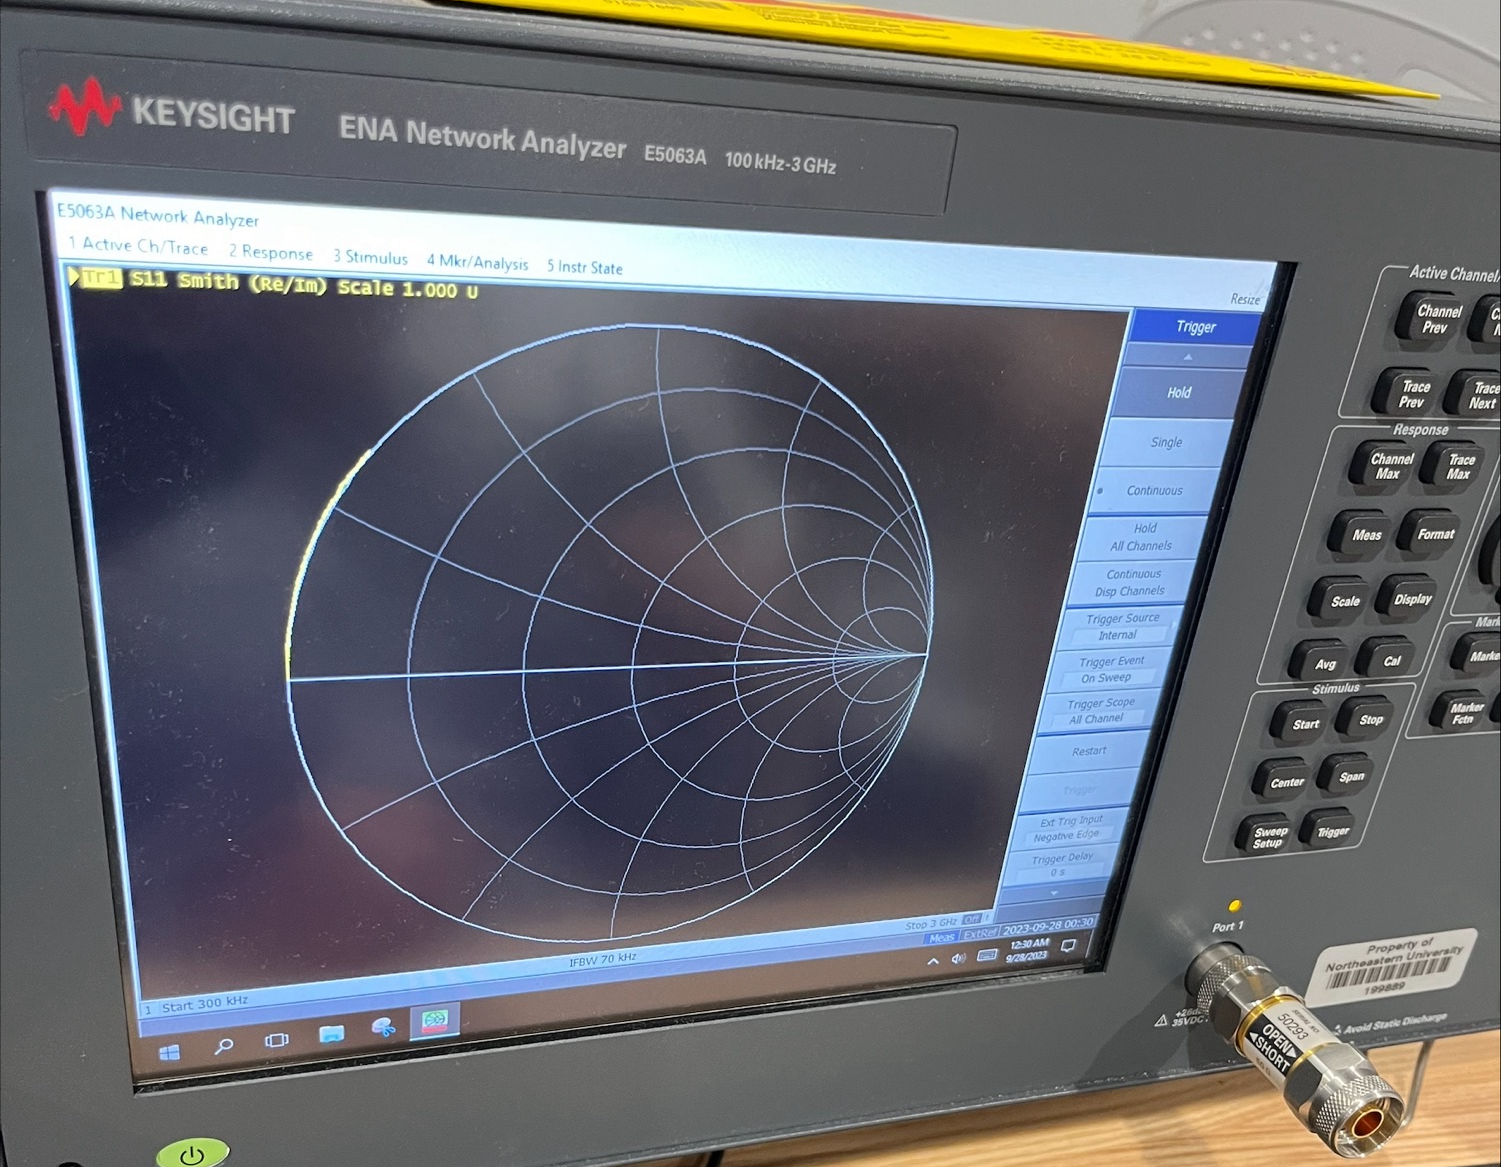
\includegraphics[width=.65\textwidth]{Figures/Lab One/ShortedLoad.png}
  \caption{Shorted Load Smith Chart}
  \label{fig:1}
\end{figure}

\begin{figure}[H]
  \centering
  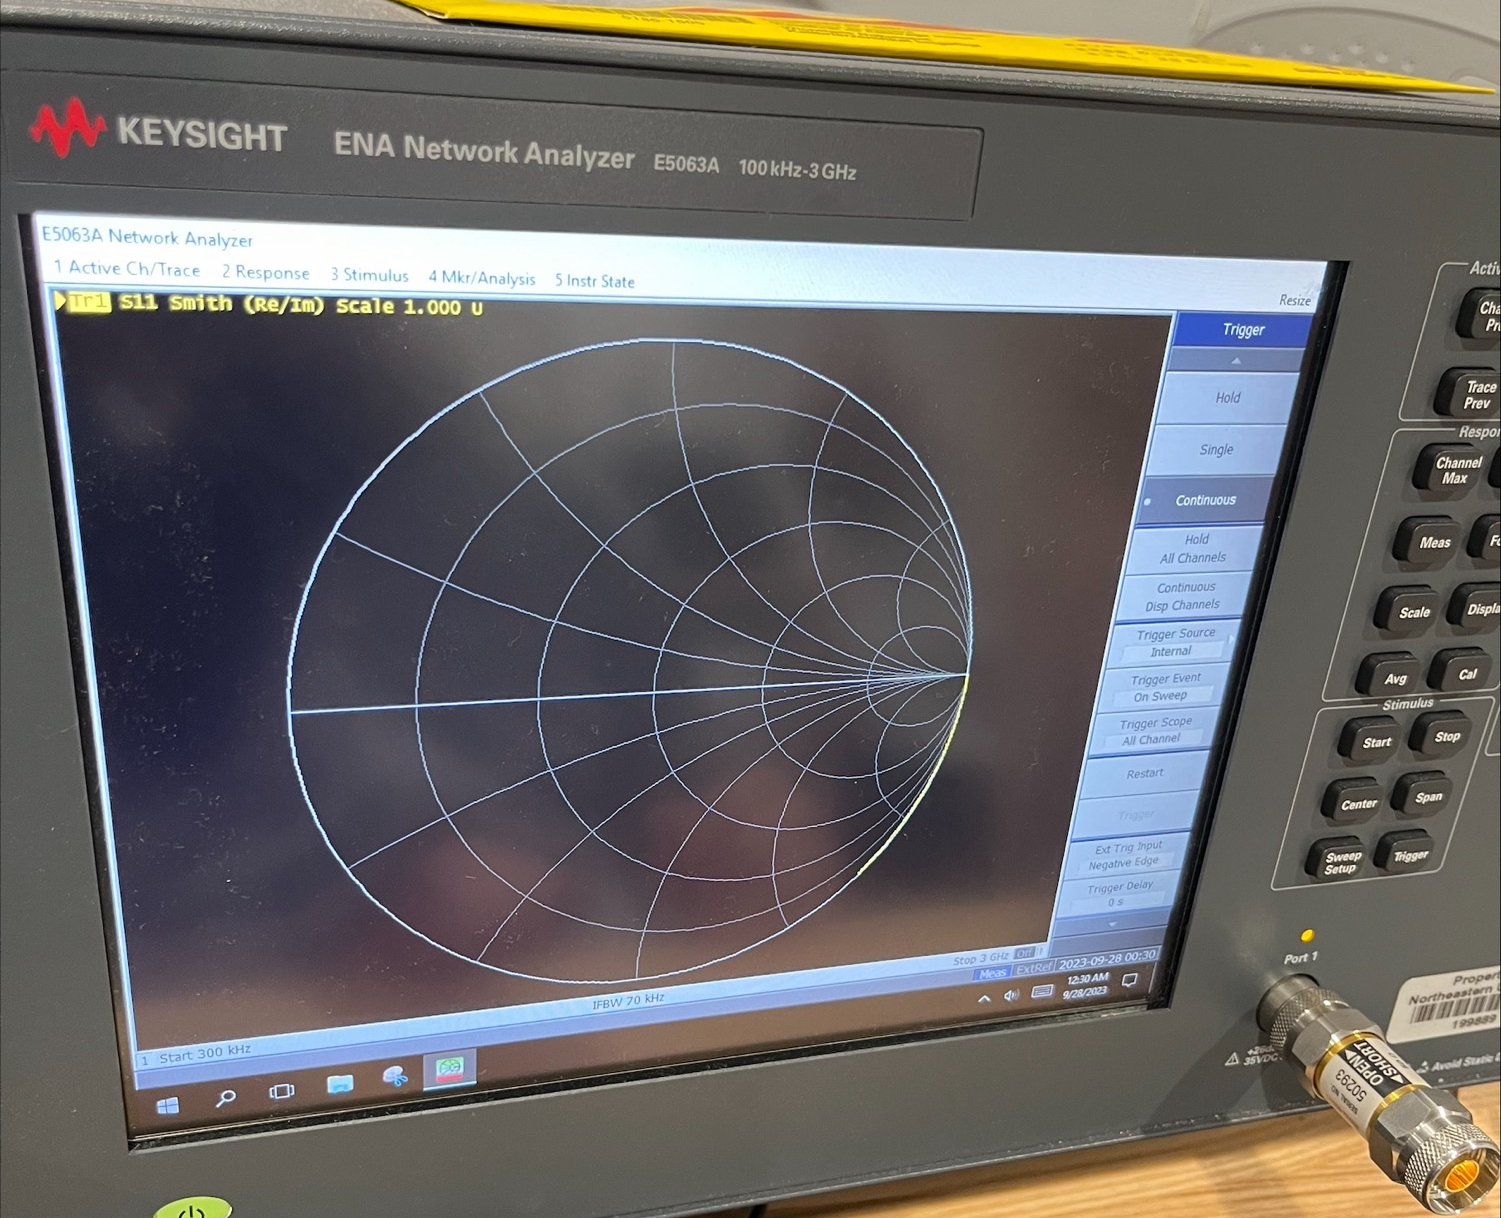
\includegraphics[width=.65\textwidth]{Figures/Lab One/OpenLoad.png}
  \caption{Open Load Smith Chart}
  \label{fig:2}
\end{figure}

\begin{figure}[H]
  \centering
  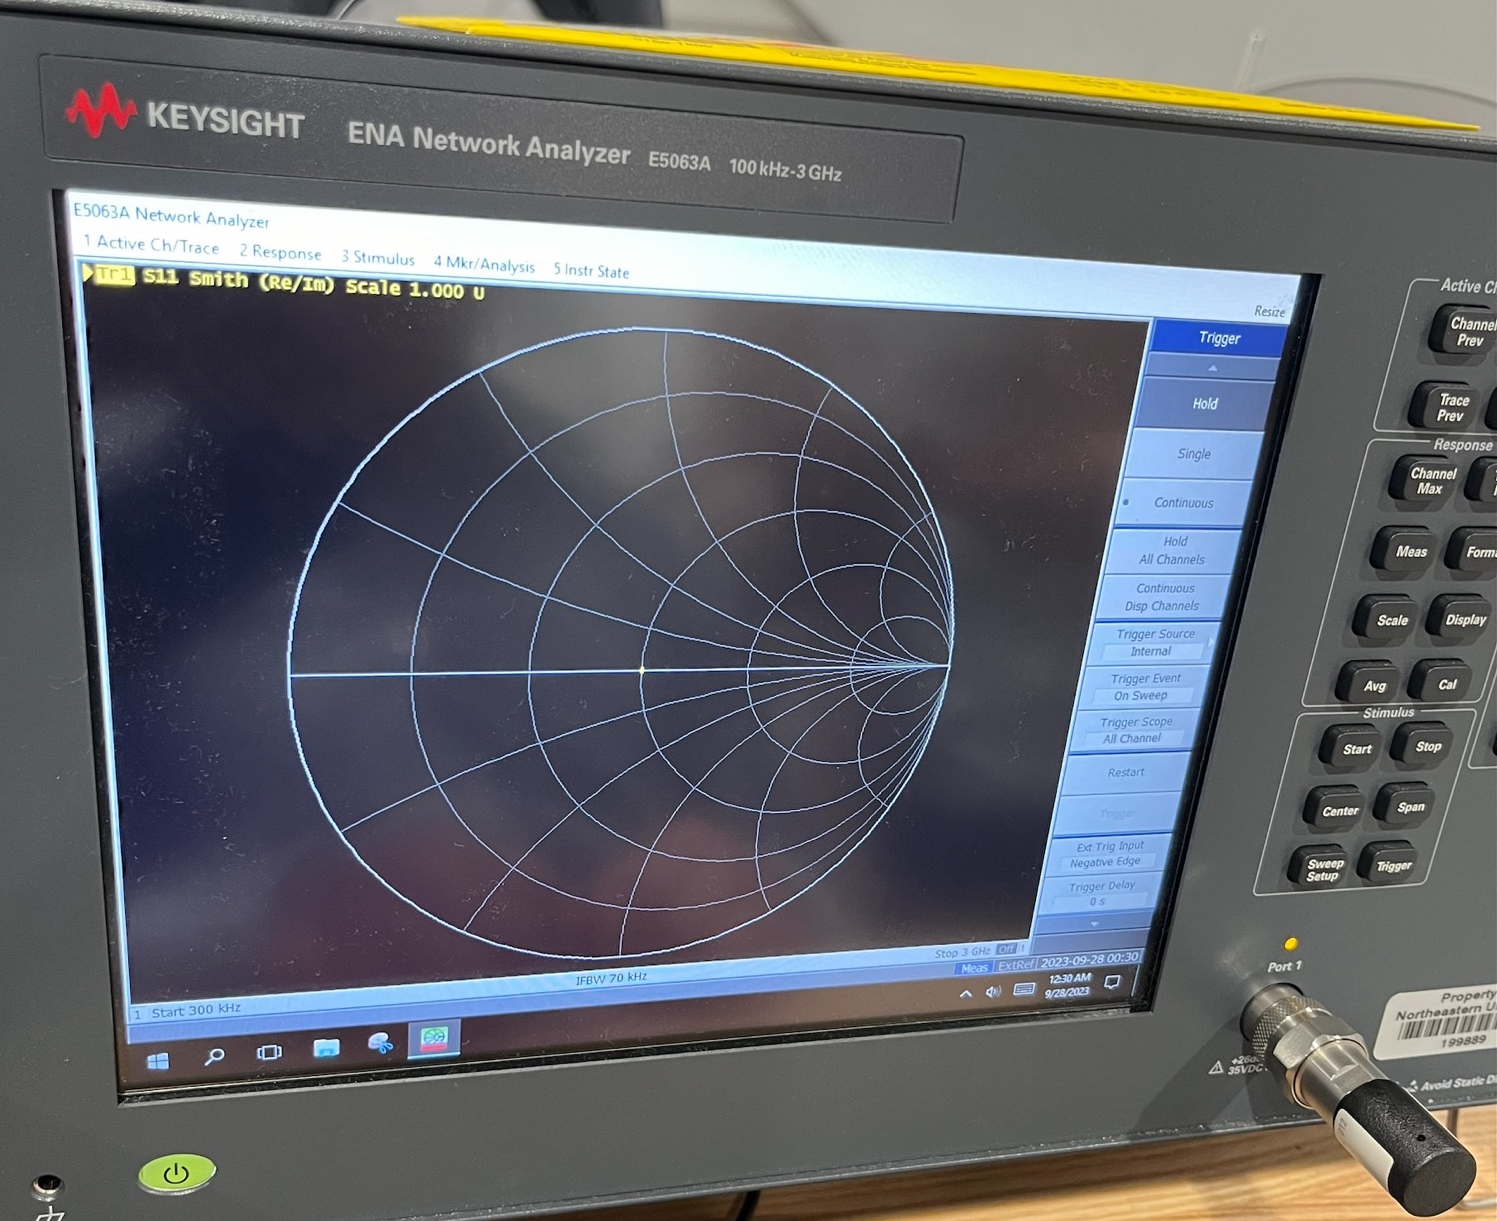
\includegraphics[width=.65\textwidth]{Figures/Lab One/MatchedLoad.png}
  \caption{Matched Load Smith Chart}
  \label{fig:3}
\end{figure}

Evidently, we see the behavior is exactly as expected; that is, the shorted load appears at the top left of the Smith chart, with slight variation, and the opened load appears at the bottom right, with some variation. The matched load, on the other hand, occurs right at the center of the chart, as it should when the impedance is matched.\\

We then used this data to estimate the length of the transmission line inside of the network analyzer, $\Delta z$, assuming the speed of light in the transmission line as $c$. As shown in Figure \ref{fig:4} below, the phase shift is roughly $67.87^{\circ}$ — we rounded to $70^{\circ}$.\footnote{As a continuous sweep, the phase would jump from roughly 60 to 80 degrees; thus, 70 seemed an appropriate estimate}

\begin{figure}[H]
  \centering
  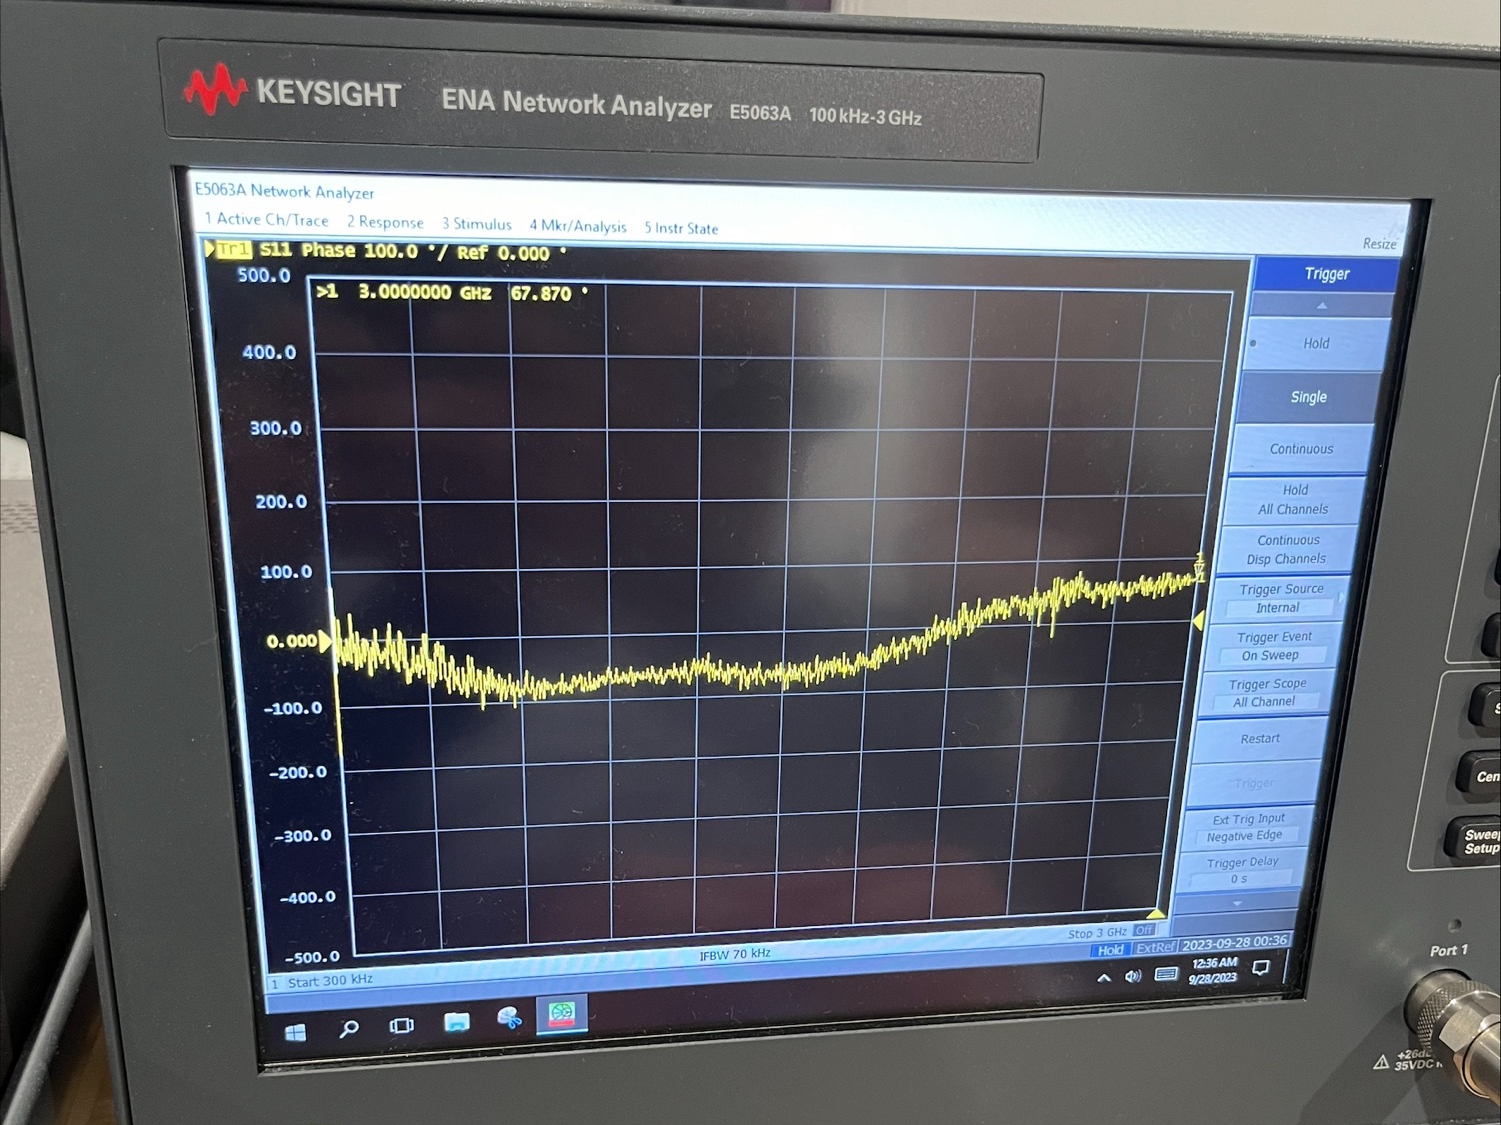
\includegraphics[width=.65\textwidth]{Figures/Lab One/MatchedPhase.png}
  \caption{Phase for Matched Load}
  \label{fig:4}
\end{figure}

The calculation performed began with the formula

$$e^{-j\theta}=e^{-2j\beta\Delta z}$$
$$\theta=2\beta\Delta z$$
$$\Delta z=\frac{\theta}{2\beta}$$

In terms of radians, we found $\theta$ as:

$$\frac{70\cdot2\pi}{360}=1.2217[\text{rad}]$$

We know $\beta=2\pi/\lambda$, and $\lambda=c/f$. Substituting gives us:

$$\Delta z = \frac{\theta c}{4\pi f}$$

Using the values we have, we get:

$$\Delta z=\frac{(70)(3\cdot10^8)}{4\pi(3\cdot10^9)}=9.97\cdot10^{-3}[\si{\meter}]\approx1[\si{\centi\meter}]$$

We now connect the BNC adapter. With an open-circuit BNC, we obtain the Smith chart shown in Figure \ref{fig:5}:

\begin{figure}[H]
  \centering
  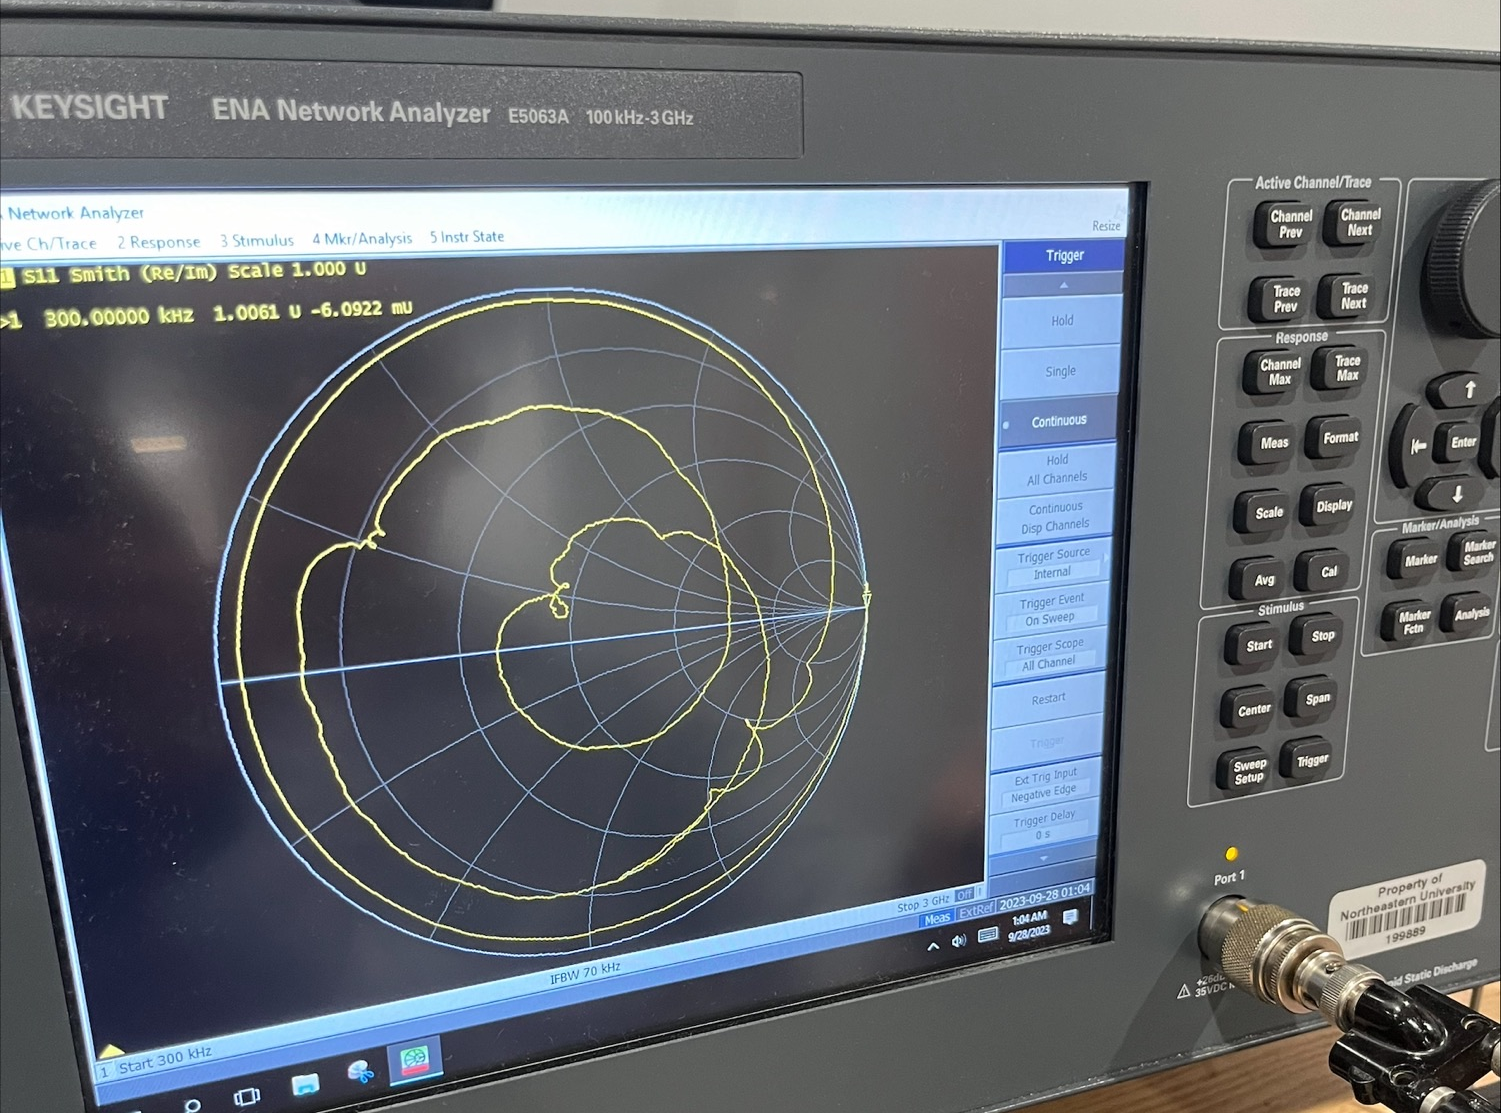
\includegraphics[width=.75\textwidth]{Figures/Lab One/OpenBNC.png}
  \caption{Open Load with BNC Adapted}
  \label{fig:5}
\end{figure}

We can see that the output immediately becomes more lossy than the open circuit calibration connector. This can be explained by the fact that the BNC adapter adds length to the transmission line. In doing so, more of the same wavelengths can fit, which means the wave travels farther. Thus, more of the current and voltage is lost.\\

We know plug in various components with the BNC, as described in Figures \ref{fig:6}-\ref{fig:8}:

\begin{figure}[H]
  \centering
  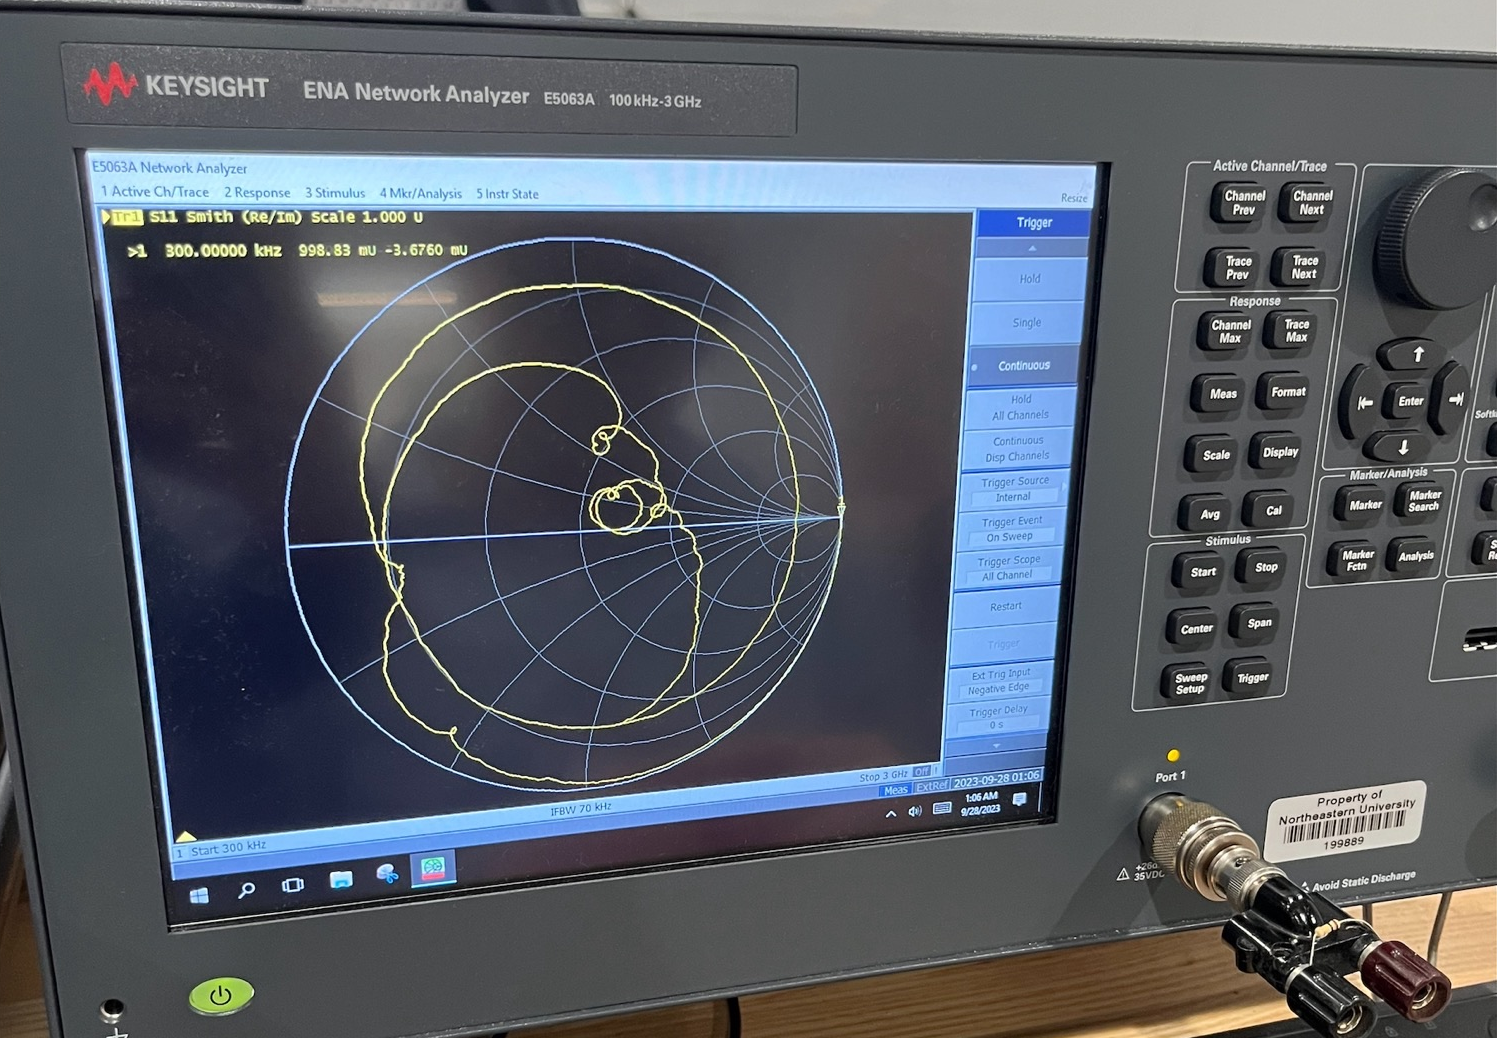
\includegraphics[width=.75\textwidth]{Figures/Lab One/ResistorBNC.png}
  \caption{BNC with Resistor}
  \label{fig:6}
\end{figure}

The resistor more or less looks as it should; that is, it starts with no impeding component; however, as the frequency increases, significant loss occurs.

\begin{figure}[H]
  \centering
  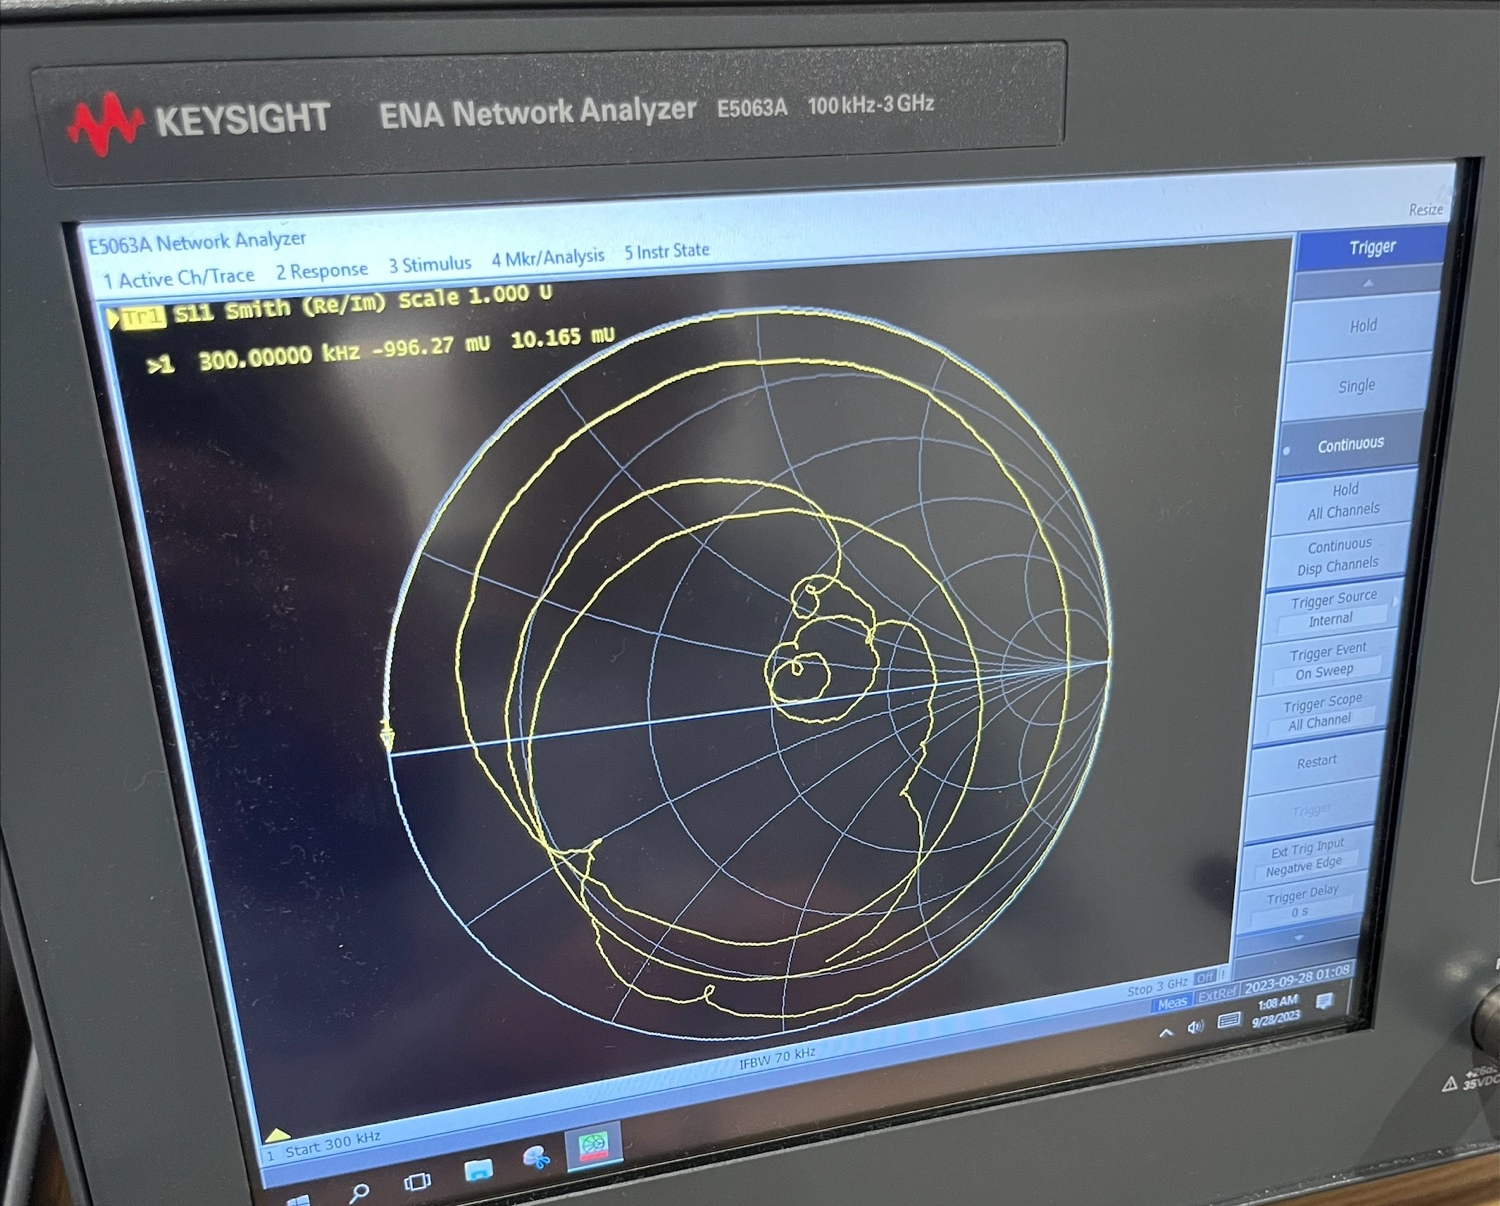
\includegraphics[width=.75\textwidth]{Figures/Lab One/CapacitorBNC.png}
  \caption{BNC with Capacitor}
  \label{fig:7}
\end{figure}

At lower frequencies, the capacitor appears as it should — it is following an impedance proportional to $-\frac{j}{\omega C}$. As the frequency increases, however, a loss occurs, as indicated by the spiral. This can be explained by the fact that capacitors begin as open circuits, but, at high frequencies, capacitors act as short circuits.

\begin{figure}[H]
  \centering
  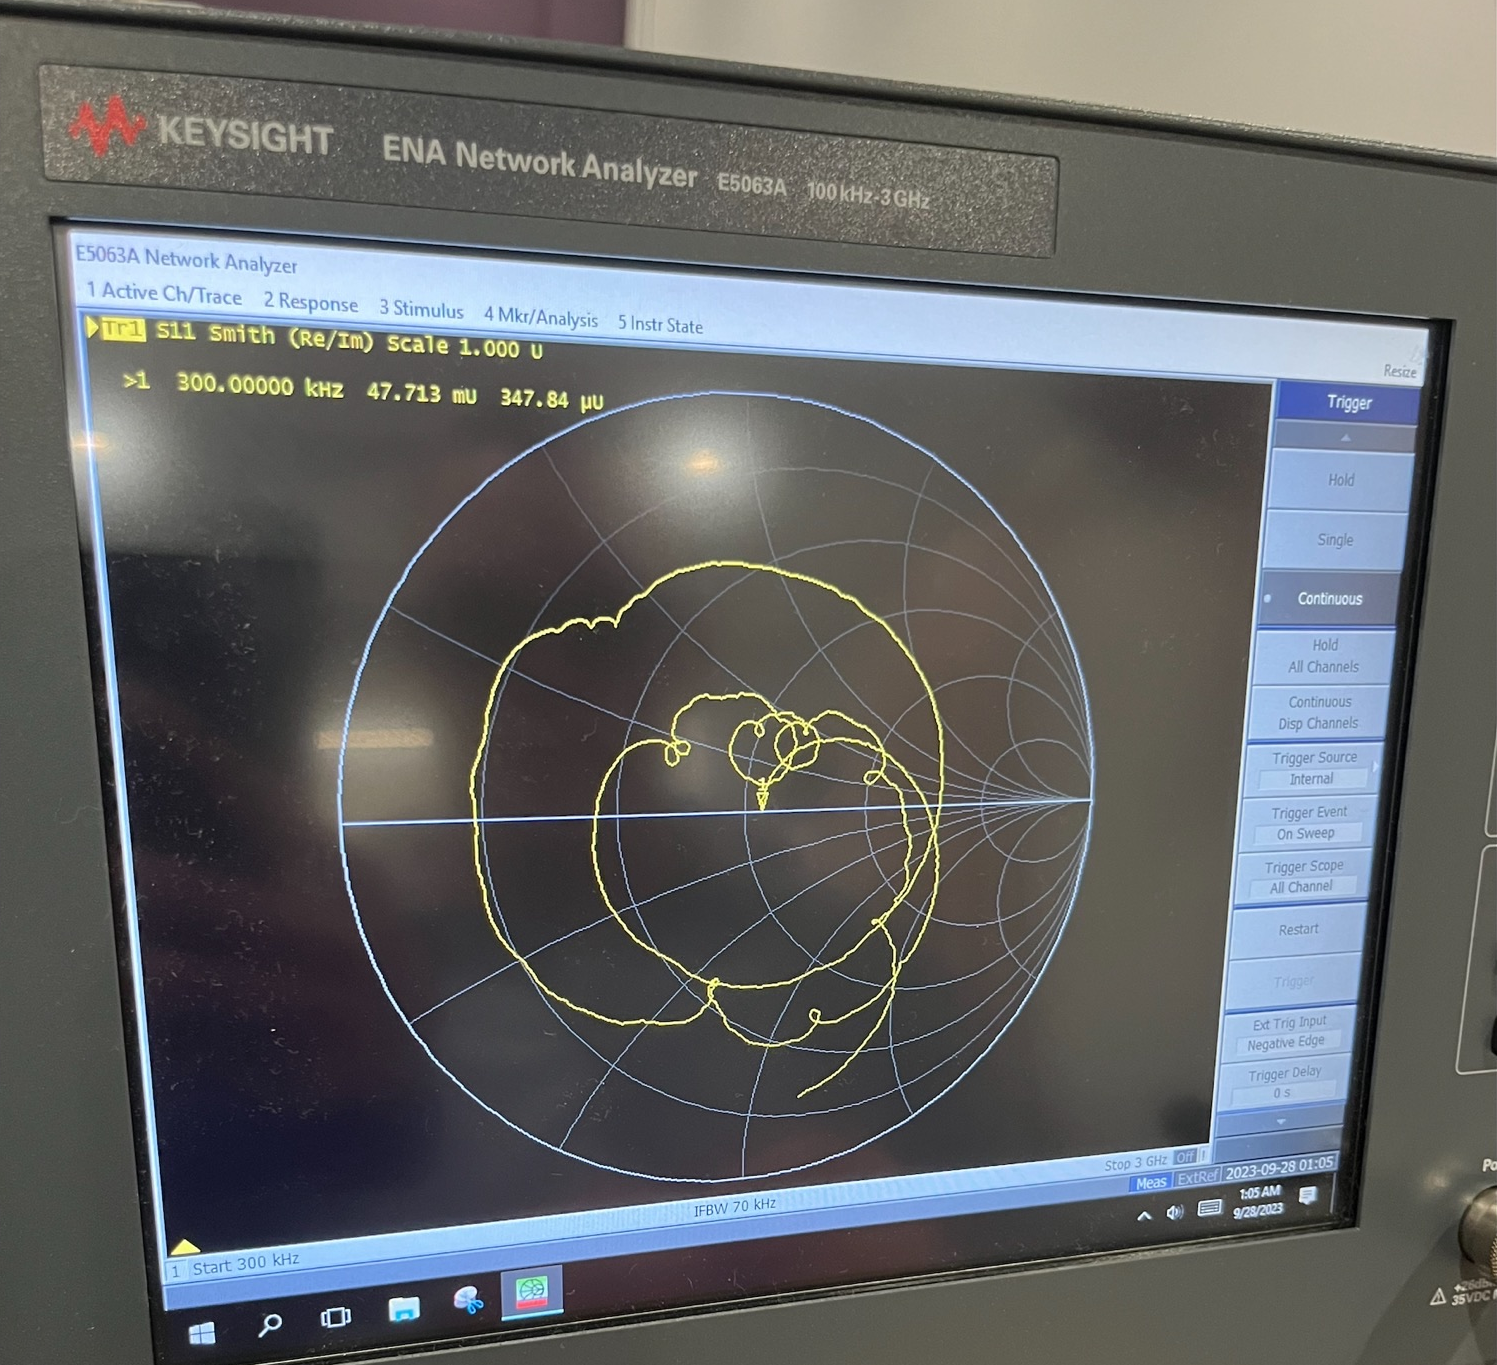
\includegraphics[width=.75\textwidth]{Figures/Lab One/InductorBNC.png}
  \caption{BNC with Inductor}
  \label{fig:8}
\end{figure}

In the picture above, the inductor doesn't behave exactly as expected; this is most likely because it was not coiled tight enough. We do see, however, a tendency for lossiness as the frequency increases.\\

After this, we plug in a short and long wire, as shown in Figures \ref{fig:9} and \ref{fig:10}:

\begin{figure}[H]
  \centering
  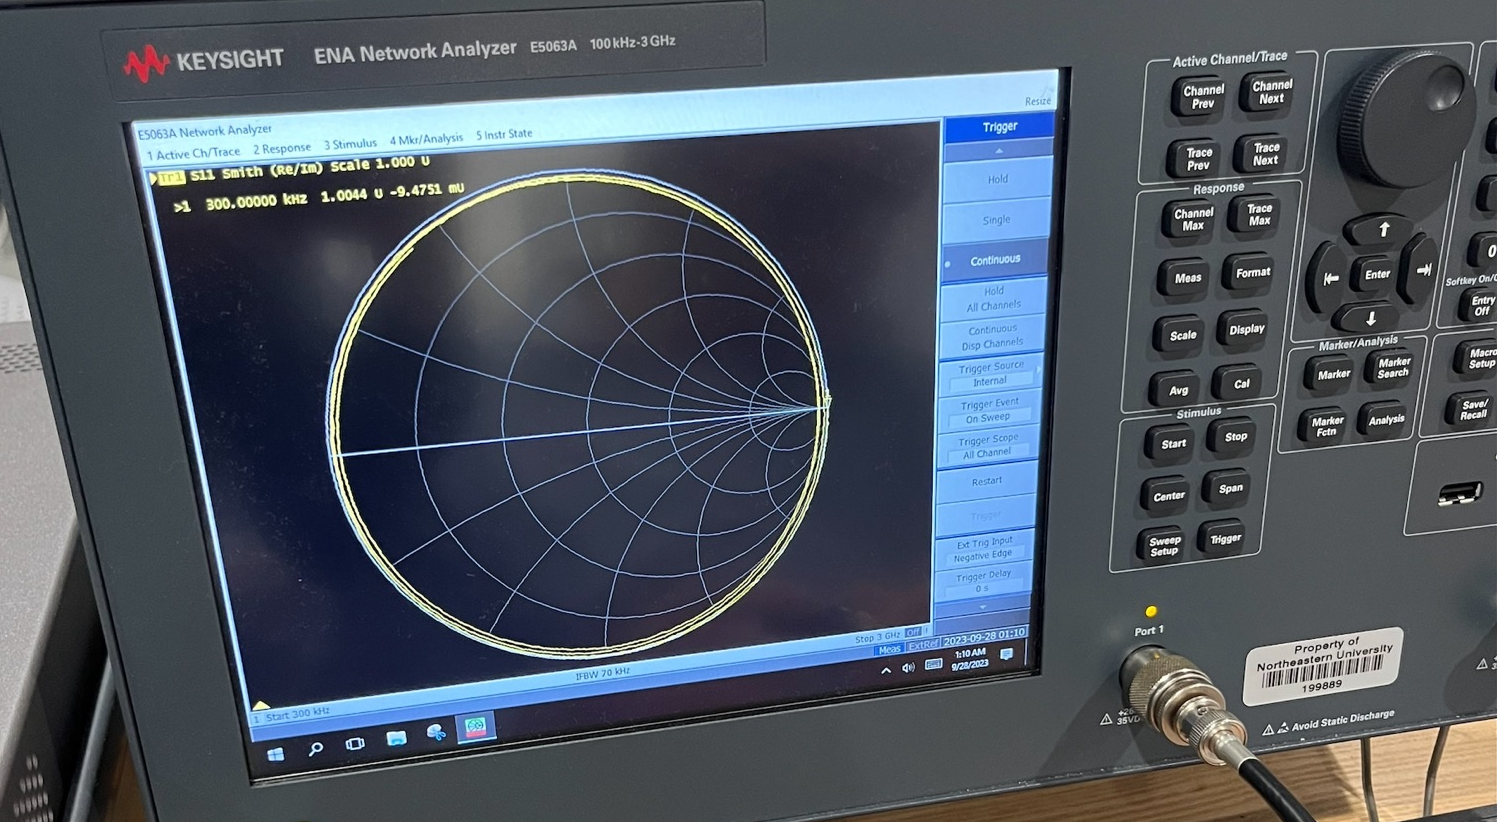
\includegraphics[width=.75\textwidth]{Figures/Lab One/ShortWire.png}
  \caption{The Short Wire}
  \label{fig:9}
\end{figure}

\begin{figure}[H]
  \centering
  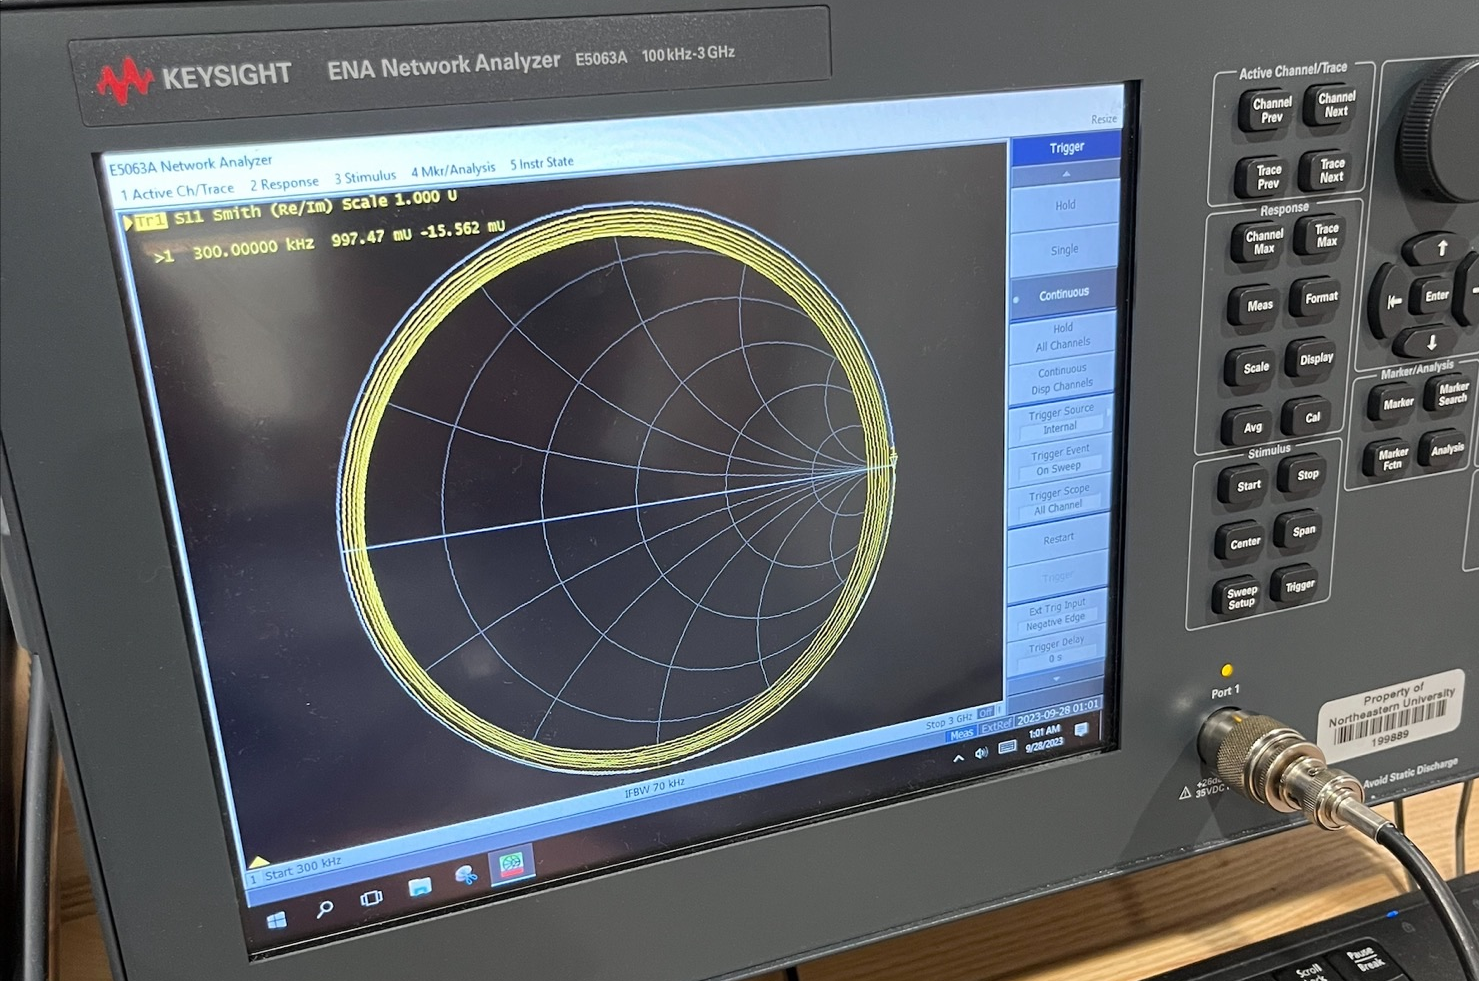
\includegraphics[width=.75\textwidth]{Figures/Lab One/LongWire.png}
  \caption{The Long Wire}
  \label{fig:10}
\end{figure}

We see that, with the longer cable, the Smith chart has more ``rings'' or loops. Logically, this makes sense. We know that a single ``loop'' is one phase/360 degrees. As a wire gets longer, it will fit more phases/wavelengths in it, and, thus, display more loops in a Smith chart. Both wires show increasing losses, as the circles spiral into the center. The length of the cable was measured as approximately $23.5[\si{\centi\meter}]$. We can then calculate the dielectric constant:

$$\varepsilon_r=\left( \frac{\lambda_o\theta_m}{4\pi\Delta z} \right)^2$$

Using the values we obtained for the longer wire, we get:

  $$\varepsilon_r=\left(\frac{(.1)(7.5\text{ cycles})}{4\pi(.235 + .01)}\right)^2$$
  $$\varepsilon_r=\left(\frac{(.1)(47.124[\text{rad}])}{4\pi(.245)}\right)^2=2.34$$

  Now analyzing the amplitude, phase, and Smith outputs for a matched load, we find the outputs shown in Figures \ref{fig:11}-\ref{fig:13}:

  \begin{figure}[H]
    \centering
    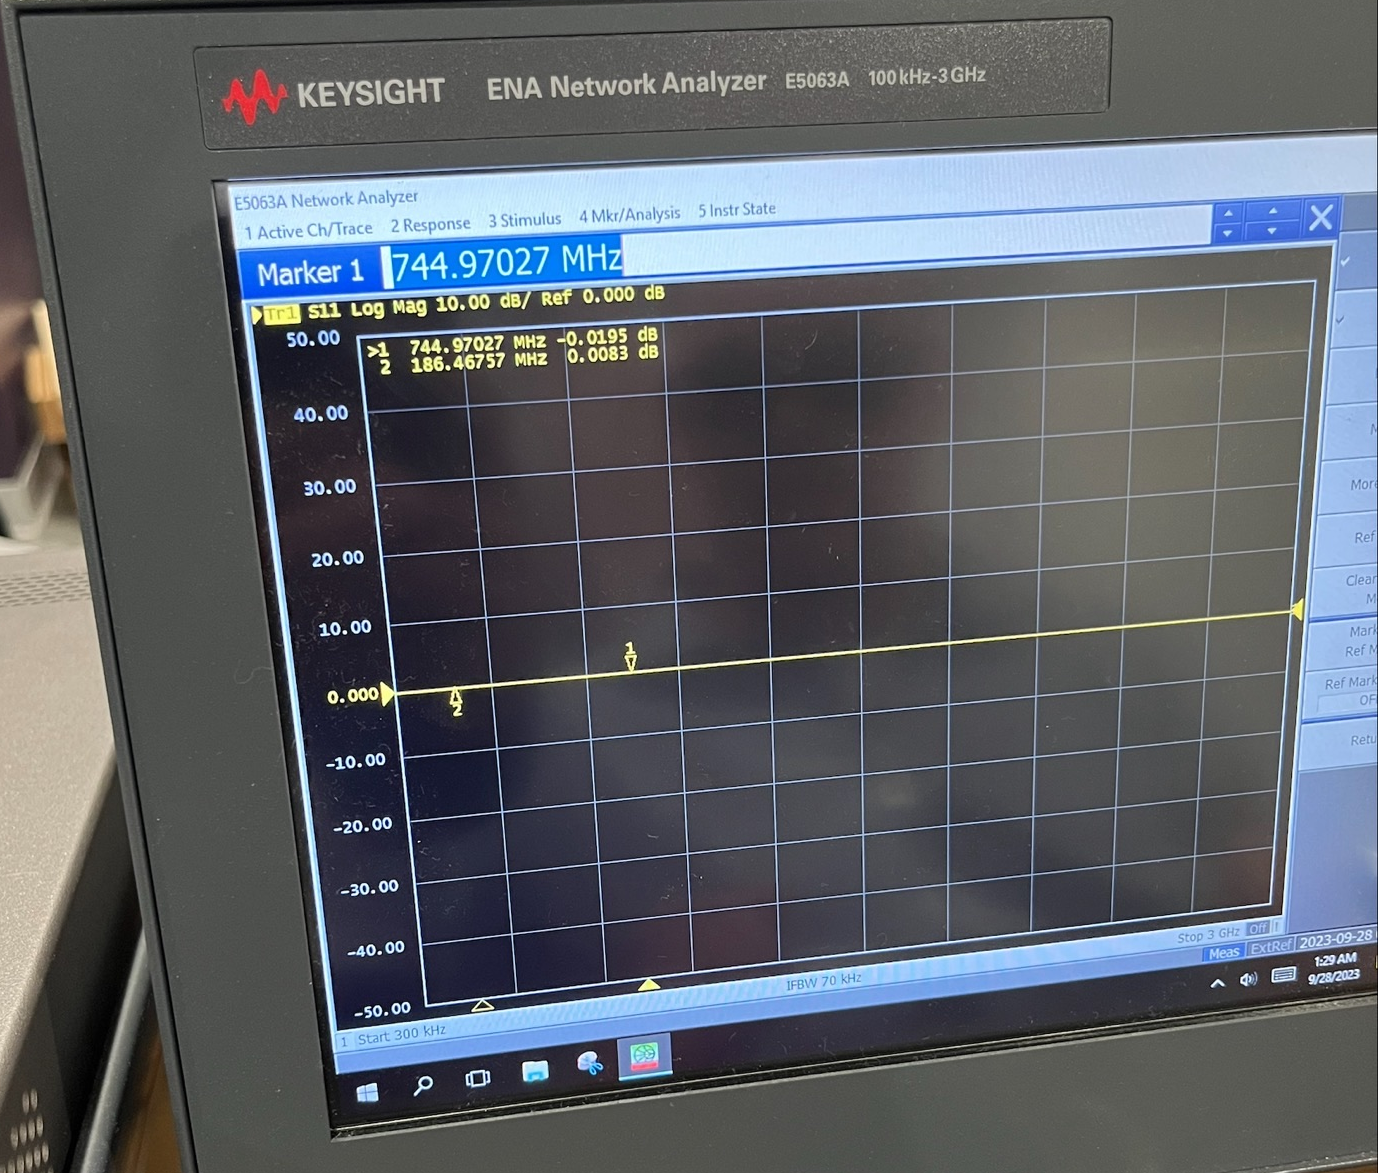
\includegraphics[width=.75\textwidth]{Figures/Lab One/Amp.png}
    \caption{The Amplitude Display with Log Magnitude}
    \label{fig:11}
  \end{figure}

  \begin{figure}[H]
    \centering
    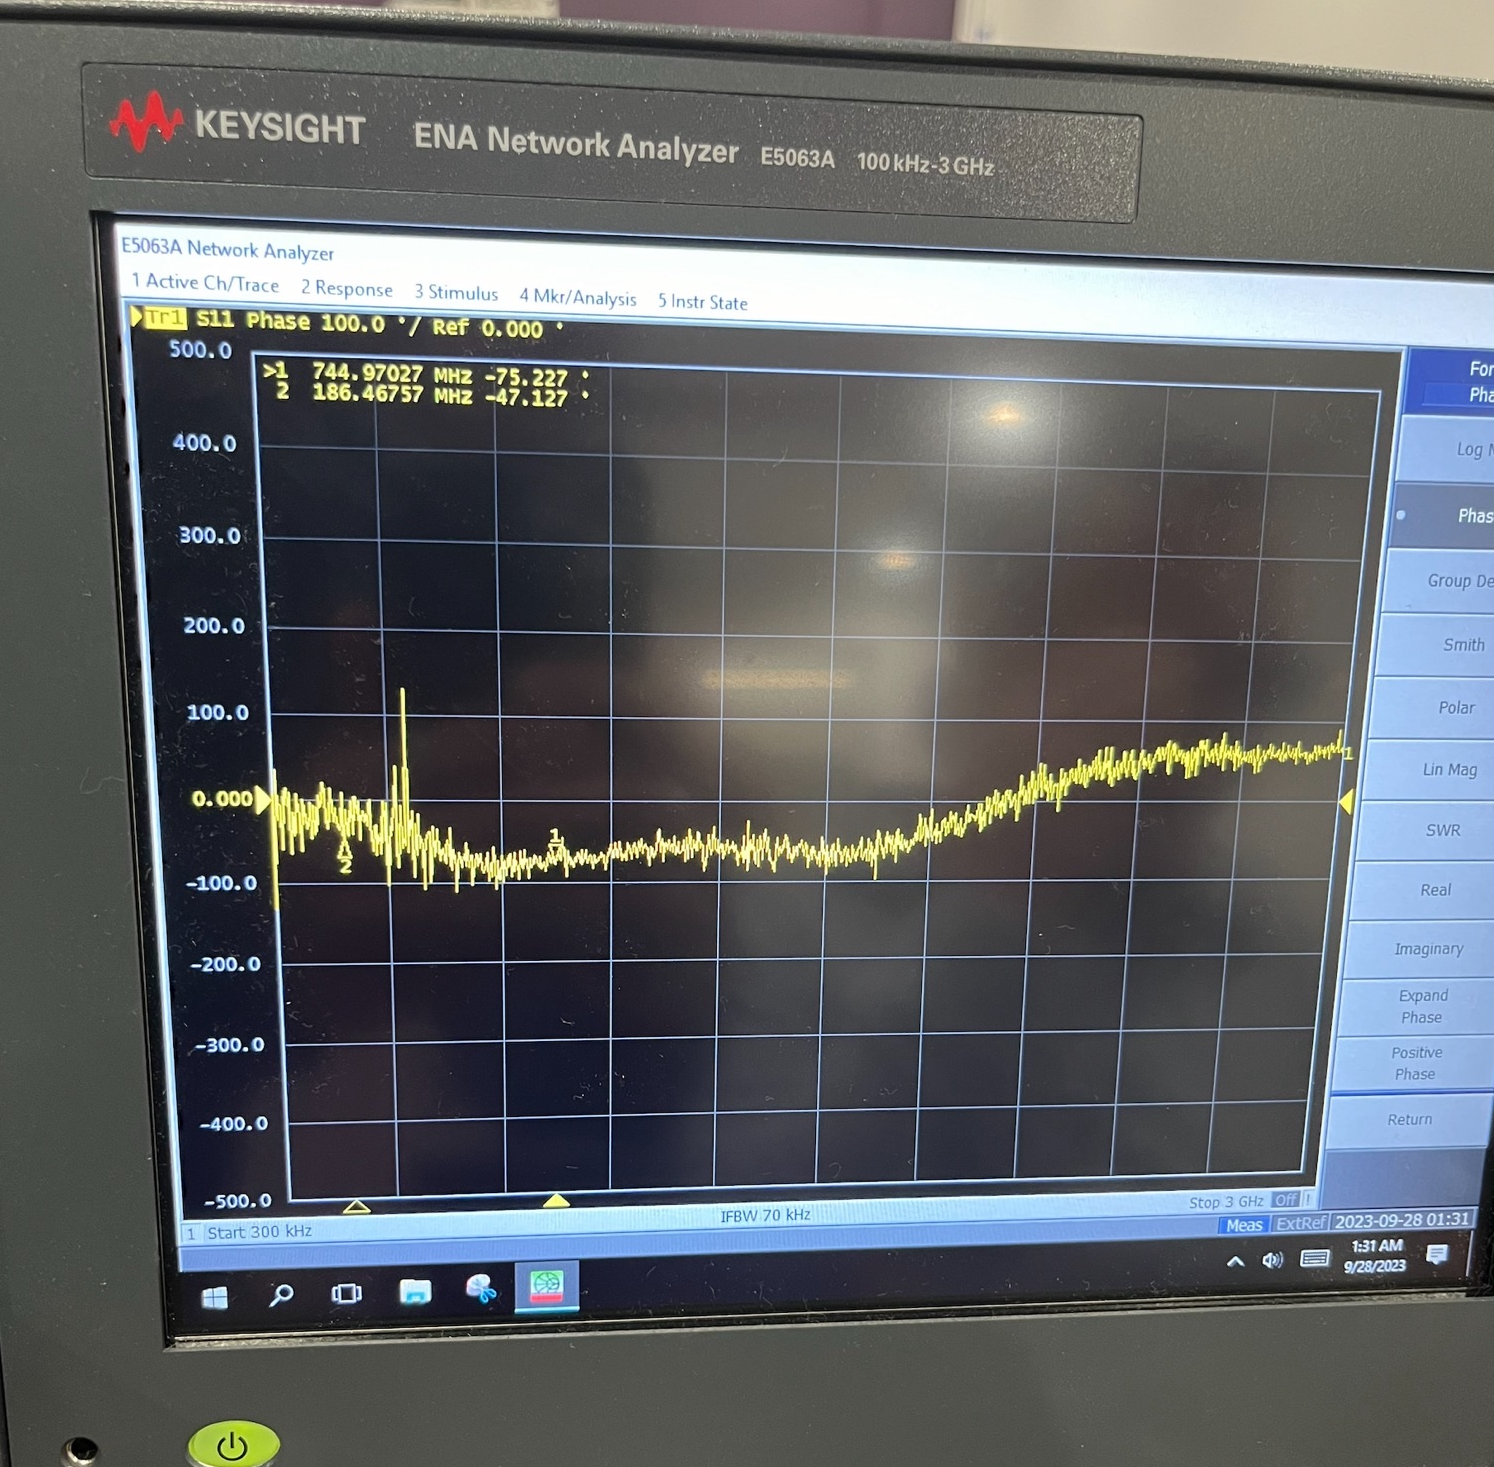
\includegraphics[width=.75\textwidth]{Figures/Lab One/Phase.png}
    \caption{The Phase Display}
    \label{fig:12}
  \end{figure}

  \begin{figure}[H]
    \centering
    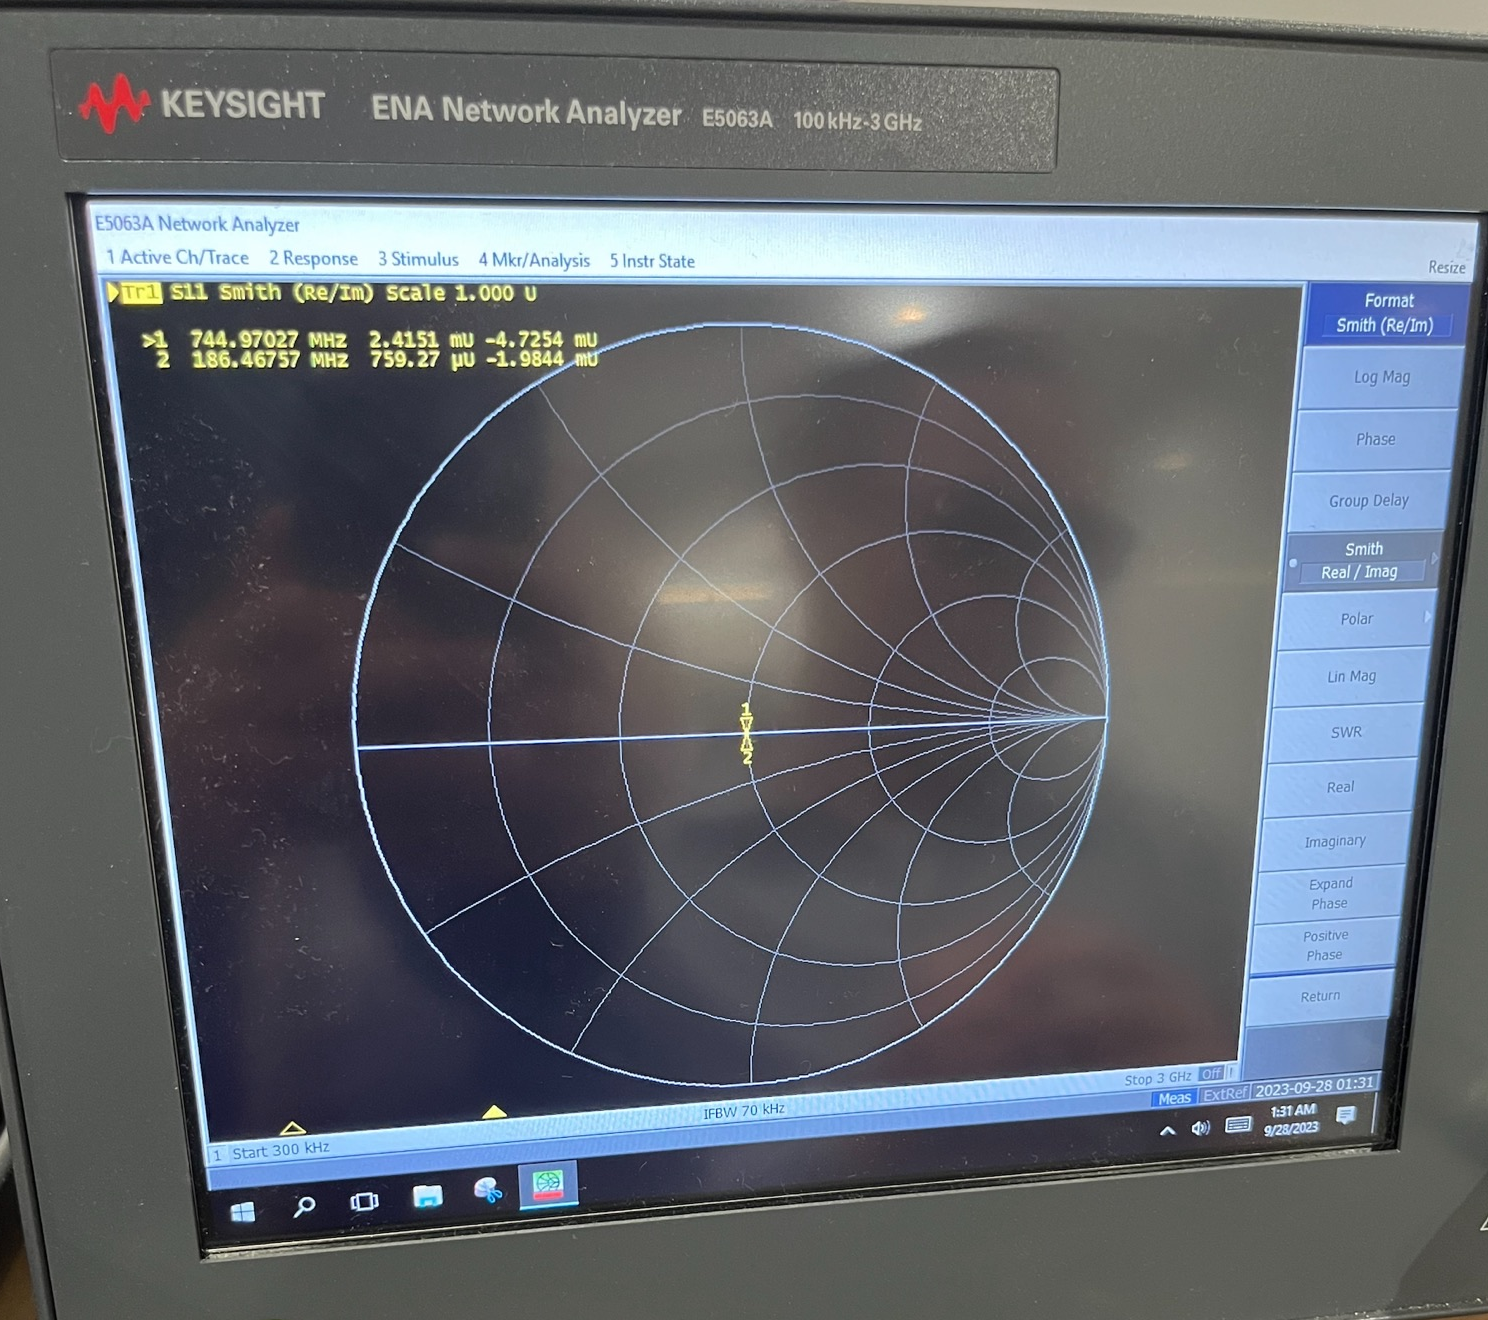
\includegraphics[width=.75\textwidth]{Figures/Lab One/Smith.png}
    \caption{The Smith Chart Display}
    \label{fig:13}
  \end{figure}

  Overall, the most graphically concise (that is, most information in simplest format) chart seems to the Smith chart. Though it depends on exact purpose (like, sometimes, the phase display can more easily show the phase angle), the Smith chart seems the best tool.

\section{Conclusion}

\end{document}
